\documentclass[tikz,border=10pt]{standalone}
\usepackage{tikz}
\usepackage{amsmath}  % <-- needed for \text
\usetikzlibrary{arrows.meta, positioning, backgrounds, fit}
\newcommand{\textdot}[1]{\ensuremath{\dot{\text{#1}}}}

\begin{document}
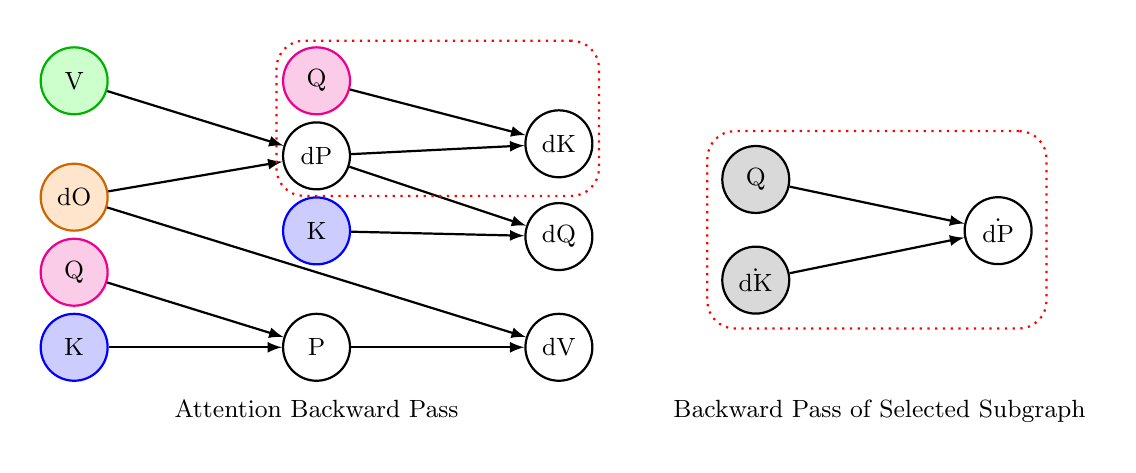
\begin{tikzpicture}[
    >=latex,                  % Use LaTeX arrow tips
    every edge/.style={->, thick, draw=black},  % Black arrows
    node distance=1.8cm,       % Vertical spacing between “below=...”
    thick,  show background rectangle,               % Tells TikZ to
    % draw the background rectangle
    background rectangle/.style={fill=white} % Sets the background
    % rectangle fill color to white
  ]

  %--- Colored styles for Q, K, V, dO ---
  \tikzset{
    titleStyle/.style   ={rectangle, draw=white, fill=white, thick,
    font=\small},
    Qstyle/.style   ={circle, draw=magenta, fill=magenta!20, thick,
    minimum size=8.5mm, font=\small},
    Kstyle/.style   ={circle, draw=blue, fill=blue!20, thick, minimum
    size=8.5mm, font=\small},
    Vstyle/.style   ={circle, draw=green!70!black, fill=green!20,
    thick, minimum size=8.5mm, font=\small},
    dOstyle/.style  ={circle, draw=orange!80!black, fill=orange!20,
    thick, minimum size=8.5mm, font=\small},
    % White style for all other nodes
    whiteNode/.style={circle, draw=black, fill=white, thick, minimum
    size=8.5mm, font=\small},
    whiteNode2/.style={circle, draw=black, fill=gray!30!white, thick, minimum
    size=8.5mm, font=\small},
  }

  %------------------------------------------------------------------------------
  % 1) First column (colored)
  %    V, dO, Q, K (top to bottom)
  %------------------------------------------------------------------------------
  \node[Vstyle]  (V)  at (0,0)    {V};
  \node[dOstyle] (dO) [below=.6cm of V]  {dO};
  \node[Qstyle]  (Q1) [below=.075cm of dO] {Q};

  \node[Kstyle]  (K1) [below=.075cm of Q1] {K};

  %------------------------------------------------------------------------------
  % 2) Second column (white)
  %    Q, dP, K, P (top to bottom)
  %------------------------------------------------------------------------------
  \node[Qstyle] (Q2) [right=2.2cm of V]  {Q};
  \node[whiteNode] (dP) [below=.075cm of Q2] {dP};
  \node[Kstyle] (K2) [below=0.075cm of dP] {K};
  \node[whiteNode] (P)  [right=2.2cm of K1] {P};

  %------------------------------------------------------------------------------
  % 3) Third column (white)
  %    dK, dQ, dV (top to bottom)
  %------------------------------------------------------------------------------
  % \begin{scope}[yshift=cm]
  \node[whiteNode] (dK) [right=2.2cm of Q2, yshift=-0.8cm]  {dK};
  \node[whiteNode] (dQ) [below=.3cm of dK]  {dQ};
  \node[whiteNode] (dV) [right=2.2cm of P]  {dV};

  \node[whiteNode2] (Q3) [right=4.7cm of dP, yshift=-0.3cm]  {Q};
  \node[whiteNode2] (dotdK) [below=.4cm of Q3]  {\textdot{dK}};
  \node[whiteNode] (dotdP) [right=2.2cm of Q3, yshift=-0.65cm]  {\textdot{dP}};

  \node[titleStyle] (titleleft) [below=0.1cm of P]  {Attention Backward Pass};
  \node[titleStyle] (titleleft) [below=0.1cm of P, xshift=7.15cm]
  {Backward Pass of Selected Subgraph};

  %------------------------------------------------------------------------------
  % Edges requested:
  %   V -> dP
  %   dO -> dP
  %   Q (col 1) -> P
  %   K (col 1) -> P
  %------------------------------------------------------------------------------
  % \draw[->, >=latex, shorten >=2pt, shorten <=2pt] (V) -- (dP);
  \draw[->, >=latex] (V)  -> (dP);
  \draw[->, >=latex] (dO)  -> (dP);
  \draw[->, >=latex] (Q1)  -> (P);
  \draw[->, >=latex] (K1)  -> (P);

  \draw[->, >=latex] (Q2)  -> (dK);
  \draw[->, >=latex] (dP)  -> (dK);
  \draw[->, >=latex] (dP)  -> (dQ);
  \draw[->, >=latex] (K2)  -> (dQ);

  \draw[->, >=latex] (dO)  -> (dV);
  \draw[->, >=latex] (P)  -> (dV);

  \draw[->, >=latex] (Q3)  -> (dotdP);
  \draw[->, >=latex] (dotdK)  -> (dotdP);

  % \draw[red, thick, dotted] plot [smooth cycle]
  % coordinates {(Q2) (dK) (dQ) (K2)};

  \node[
    draw=red,
    dotted,
    thick,
    rounded corners=10pt,
    fit=(Q2)(dP)(dK),
    inner sep=2pt  % Extra padding so the node circles all lie inside
  ] {};

  \node[
    draw=red,
    dotted,
    thick,
    rounded corners=10pt,
    fit=(Q3)(dotdK)(dotdP),
    inner sep=5pt  % Extra padding so the node circles all lie inside
  ] {};

\end{tikzpicture}
\end{document}
